\chapter{Background}
\section{Natural Language Processing}
In order to have an understanding of the current issues arising in the process of a chatbot several areas must be understood for the current work. For instance understanding the basics of natural language processing can give us a background on how the google algorithm of Dialogflow works.

The rational behind Natural Language Processing regards to a machine learning principle which relies on computing closeness between words and correlations with others to identify patterns and generate useful test sets. This area aims to divide language processing into three areas: bag of words, bag of concepts and bag of narratives. Each of this aspects aims to connect and find a pattern between words itself which is proven to be hard by Cambria \cite{nlp_reference}. On the other hand, combinations between bags of words and bag of concepts seem to infers better the context in which sentences can help to identify and predict the next sentence. Thus, NLP algorithms use a large set of data to combine word and context syntax to allow for an ease of linking between sentences. Finally, the bag of narratives aims to combine paragraphs in order to get connected contexts, this in principle is rather hard and usually done using statistical analysis to approach patterns among sets of sentences. 

The best way to provide NLP algorithms that aim to extract not only word but also context and narrative are algorithms that simulate the human Psyche, thus deep-learning and Machine Learning algorithms that can aim to gather enough information to extract sentiments from the context and map sentences to actions and entities that allow to infers the context to provide a better word accuracy ratio as described by Cambria \cite{nlp_reference}. Using machine learning techniques to abstract and extract entities and context we can further the models and allow mapping and identification of elements that can be used and is used in transfer learning algorithms. This can be seen in DialogFlow as the tool's base maps entities, contexts and intents in order to identify sentences and break them down to identify elements and reply accordingly.

Based on the information extracted from Cambria \cite{nlp_reference} and the google white-paper \cite{nlp_deep_google} is clear that a large corpus of data or text can help to infer the context from in which it belongs and thus allowing a easier mapping of the narrative within the context allowing the extraction of entities to be perform in an accurate way. This could be combined with other methods of machine learning like reinforced learning to train a corpus of text and enrich it with interactions and allow an accurate mapping.

\section{Chatbots}

In order to understand how a chatbot work, it's important to mention that chatbots are in a constant increase and several chatbots pre-trained with big data-sets and undergoing active supervised learning are experiencing a significant growth. So is that we have the main technology companies investing a quantifiable amount of money into developing their products. This is easier understood by mapping each product to the company such as DialogFlow and Google, AmazonLex and Amazon or Luis and Microsoft. Regardless, this leaves behind the fact that some big competitors such as IBM with Watson are ahead but in practice the results seem to differ.

\begin{figure}[h]
    \centering
    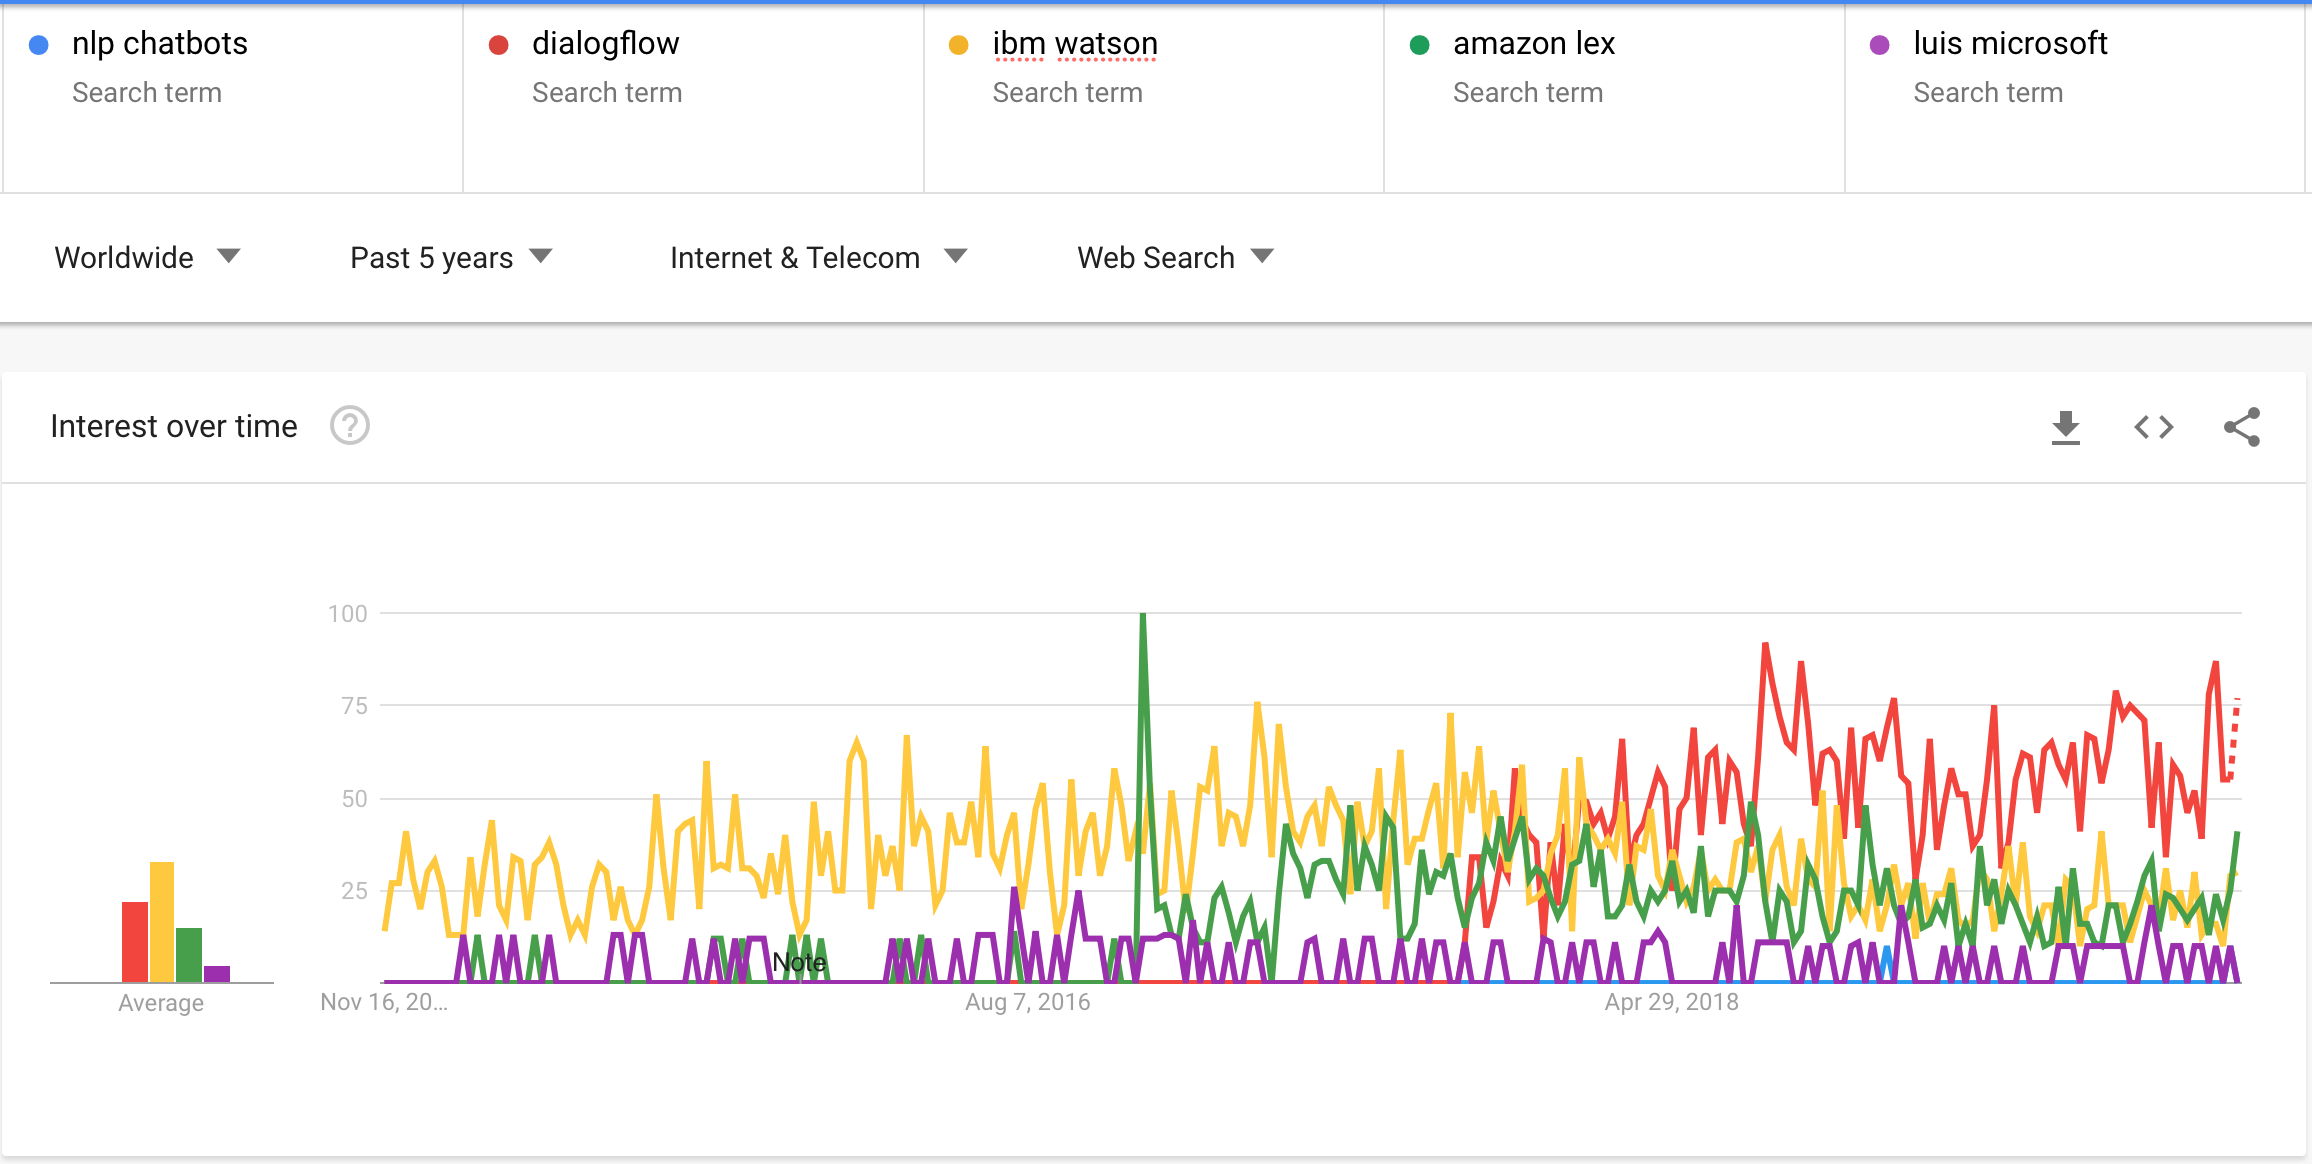
\includegraphics[scale=0.45]{MA-BA-Thesis/NLP_Chatbot_Comparison.png}
    \caption{Comparison of Google Trends for NLP Chatbots}
    \label{fig:nlp_chatbot_graph}
\end{figure}

This trend of growth among the different areas can be described in the figure \ref{fig:nlp_chatbot_graph} where we can see that there is an ongoing trend for DialogFlow over other chatbots despite the continuous big interest overtime in IBM's Watson.

\begin{itemize}
    \item Non-programming chatbots
    \item Conversation-Oriented chatbots 
    \item Platforms by tech giants' chatbots.
\end{itemize}
The breakdown of chatbots as described by Rahman\cite{chatbot_reference} describes a schema were bots are offered in different layers which include the tree based chatbots limited to answer questions and simple structures without getting into detail of the content. Then on a different layer the Conversation-Oriented chatbots use data as a foundation of information and Natural Language processing for further inspections.

In the Conversation-Oriented chatbot layer we can find that most clients have issues with training layers of data. Thus the biggest players in this category are the ones who handle and create models based on big amounts of data combined with entity and sentiment analysis. Furthermore, this leads us to the Platforms by tech gigants as described above which include DialogFlow which features pretrained models in combination with Entity and sentiment analysis which leads to ease of implementation and great gather of responses as well as context analysis.

\section{DialogFlow API}

In order to understand how the chatbot and the mappings is done its important to understand how the DialogFlow API works and what are the elements a usual chatbot looks upon before being able to convert and identify sentences into understandable machine context. To start we must understand that each sentence to be taken by the chatbot must used in two contexts, the first one to create an environment and the second to map the elements to entities in order to provide content for the chatbot to work on. To achieve this, DialogFlow uses Intents and Entitites as many other chatbots such as Rasa to extend the usability of the text recived. After the chatbot recives the text it will try to get mapped by using the trained entitites which are the words to be looked upon. For example in our case we would be looking for toolsets or problem definitions to map to unix tooling. Thus, our entities would be all the tools from the unix universe and the intent will try to comunicate the issue within this context. Additional entities can also be added and the more entities the richer the model will be. Mapping back to the example previously defined, we can say that within one intent, many entities can be mapped. To get ourselves in context we can say that the work of a text is broken into this area, despite that this will be further described in the development section to explicitly highlight the work of splitting and obtaining information from a string using a base test set.

Another important area from the DialogFlow API is the REST backend provided by google which allows us to talk back and forth with the google API to obtain the answers and also this will allow us to have structured responses since the back-end can handle JSON files. Also, the API features fulfilment which can allow us to reply using webhooks within a server app or even just to store and process a new answer using this API. Its worth mentioning that all the text will pass through the google API server. Moreover, there are additional features that will be explained during the development section that include how sentiment and entity extraction can be done in conjunction of the chat bot to further enhance the capabilities of the system. 

Finally, among the capabilities of the DialogFlow API we have composite entities and context which can aid the work of identifying subsections of entities and furthermore using the context to track a conversation within a set of responses using intents. This will be detailed in the development but is worth mentioning since most of the API is build upon this topics.

\section{Natural Language Understanding (NLU)}
what Nartual language understanding is and why do we need it.

\chapter{Related Work}
There are several related work that train to aim to recreate or at least up to certain extent achieve a similar solution as the one proposed. In order to understand one of the closest paper in terms of content and approach we can have a look at Jacob's \cite{networkIntents} paper on Refining Network Intents for Self-Driving Networks which aims to use natural language to perform entity extraction and thus allow to create intents based on the extracted entities to perform certain operations. This is quite related to our work since it used DialogFlow as a basis as well and extended its usage with an intent mapper in order to allow users which have a median or low understanding of computer networking to use and create intents based on a relatively simple pipeline which allows to create entity extraction as a service.

The process described by Jacob uses google assistant to extract entities from the utterances and pre processes them into Nile. Nile is a intent translator that aims to try to gather entity information and map this to actual intents that can be performed by and android system. Once nile has completed the task this is later on passed on to the Intent Deployer who must deploy the service itself and finally deploy a network policy based on the previous intents. Throughout the process several important areas are described, for example the machine learning model which contains Nile as a decoder. Within this area, the encoder tries to identify the input entities which are then transfered through the Thought vector to the Decoder. The Decoder will aim to create an intent based on the extracted entities and output this to the intent creator.

The intent creator is out of the scope of out work, but is worth to be mentioned as it will gather the extracted entities into a new intent that will deploy policies. This can be done using the recommending system developed by Franco \cite{MENTOR}. Related to this work we can find other interesting mappers for NLP such as Cocoon which uses first-order logic instead of machine learning for creating the intents into configurations. Moreover Cocoon lacks the capability of a operator refinement and learning the operator intent over time which leaves it behind. 

In order to understand mapping of natural languages is good to have a look at Lumi, as described by Jacobs in Deploying Natural Language Intents with Lumi in \cite{networkIntents}. In this paper we have a glimpse into information extraction, intent assembly and deployment using a tool called Lumi which is in charge of handling all the resources and routing to the right scenarios. In this area there are several other aspects that must be taken into account for our implementation such as the intention aware detection and the entity extraction that also takes place in this tool.

\section{Rasa and NLU}

An important tool to take into account before understanding why we used DialogFlow as our preferred chatbot to take into implementation instead of Rasa an opensource ChatBot that with an open source foundation. Since Rasa features NLU Natural Language Understanding which For Chatbots look into 2 elements and whose work is to look into entity extraction which allows to map further resources into either an intent description or a further entity extraction. This elements are proven by Braun \cite{nlu_complete} and the extraction of this element is also shown to be the most efficient with LUIS \cite{nlu_complete} as it shows that the corpus of the entry text usually influences on the capability of the ML algorithm to fetch and extract successfully the entity from the corpus. Despite this, NLU focuses on mapping the entitites by default on chatbots but lacks the capability of mapping certain contexts and invalidate ambiguity within the context. For example, after the corpus is delivered then a further retrieval of another intent or a successful implementation must precede and thus query a common knowledge database in order to generate a message that could hold the main elements named:

\begin{itemize}
    \item Text Planning
    \item Sentence Planning
    \item Linguistic Realizer
\end{itemize}

This elements will allow to map the original query of the user, combined with the entity extraction to a generated response that could be capable of delivering further questions to gather enough entities to satisfy the context or end the query and reply with the current information. Furthermore, neither RASA nor LUIS proved to handle the entity extraction in a very efficient manner which denotes that more work is needed in the area to correctly address the issue of entity extraction and thus allowing the chatbot to perform a complete analysis.

\section{Chatbot Technology Challenges}

In a different area we are also presented some interesting aspects of how chatbots are still limited not only by context but also by the corpus in which they work and show that there is work related to context identification but clearly addresses issues with the p-values required to accept the proposed solution by Rahman \cite{chatbot_challenges} in which three different aspects are presented that must be taken into account to understand limitations of the current state of NLU and chatbot development that might cap our project or set a logical boundary. Rahman describes that the current challenges which still hold now a days are related to how we extract information for each query. 

They propose a theory which is used in most chatbots now a days, thus we use intents to map input to contexts and once this intent is recognized we can performs entity extraction to gather the important elements from the conversation leaving aside the facts that are not crucial for the implementation. In this way, the paper introduces B-Point Tree which outperforms the BST tree used in NLP Classifiers as supervised training which is the common technique used in chatbots. With this approach it is easier to infer the context and map the entities to the intents since you may have many intents to a single context.

\section{Cybersecurity Solutions}

Sula \cite{recomendationSystem} gathered information about protection services for a subset of types of attack and generated recommendations based on this. This relates to our work as it might contain several pieces of information that help us to extend our service past the gathering of requirements and delivery of information. In his work Sula gathered a table containing a set of services and a relative reference pricerange which could be used to map possible entity extraction outcomes to possible solution tools. The table from Sula \cite{recomendationSystem} gathered the following elements:


\begin{table}[h]
\centering
\caption{Services and Pricing from Sula \cite{recomendationSystem}}
\resizebox{\textwidth}{!}{%
\begin{tabularx}{\textwidth}{|l|l|l|l}
\hline
Provider               & Service                         & Pricing                                    & Deployment              \\ 
\hline
Cloudflare             & Advanced DDoS Attack Protection & Free Trial                                 & Cloud based             \\ 
\hline
Imperva                & Incapsula                       & approx. \$3500 per month, \$5000 for setup & Cloud based             \\ 
\hline
Arbor Networks         & Arbor Cloud                     & on Request                                 & In Cloud \& On Premise  \\ 
\hline
Verisign               & DDoS Protection Service         & on Request                                 & Cloud Based             \\ 
\hline
Level 3 Communications & DDoS Mitigation                 & on Request                                 & In Cloud \& On Premise  \\ 
\hline
Corero                 & SmartWall Threat Defense System & approx. \$2500 per month, \$1000 for setup & In Cloud \& On Premise  \\ 
\hline
Flowmon                & DDoS Defender                   & Free Trial                                 & Cloud based             \\ 
\hline
Akamai                 & Kona Site Defender              & approx. \$6000 per month, \$3000 for setup & Cloud based             \\
\hline
\end{tabularx}
}
\end{table}

Here we can see a set of element that could be used to expand and use in our chatbot and can still can cause a beneficial impact on the system administrator experience. It is very important to mark that from this table not all elements are described in detail and not all solutions can be used to be mapped to all problems and thus there are underlying limitations.

Also, as it will be described later on many other services that also provide a comprehensive support system are available on the market and could be used to expand the usage of our chatbot.